\chapter{测量}

裁剪衣服要量尺寸,检查身体要称体重,赛跑竞走要测时间,诊断疾病要测体温。
我们在日常生活中经常要进行各种测量。

测量在现代生产技术和科学研究中非常重要,
一架复杂的机器,有成千上万个零件,在制造和安装这些零件的时候,都要进行准确的测量。
一只手表有 100 多个零件,每个零件都有严格的尺寸和形状,其中有的关键性零件要做得非常精密,
差一根头发丝的几分之一都不行,否则装配起来的手表就走不准。

同学们在学习物理的过程中还会体会到,测量在物理学中也十分重要。
我们学习物理,就从学习测量开始。

\section{长度的测量}\label{sec:1-1}

人们在建造铁路、房屋,计算土地面积的时候,都要测量长度。
测量长度,首先要确定一个标准长度,用标准长度去量被测的长度,才能得出被测长度的数值。
这个被确定的标准长度叫做\CJKunderwave{长度单位}。

世界各国原来使用的长度单位很不相同,例如,在我国用市尺,在英、美等国用英尺。
后来为了便于科学技术的交流,国际上规定了一套统一的单位,叫做\textbf{国际单位制},
已经被包括我国在内的许多国家采用。在今后学习中,我们将主要使用国际单位制。
在国际单位制中,长度的主单位是\textbf{米}(也叫公尺)。

用米作单位,北尔到哈尔滨的铁路长度大约是 1 388 000 米,这种写法数字较大;
物理课本中一张纸的厚度,大约是 0.000 075 米,这种写法数字又太小。
数字太大或太小,读和写都不方便。因此,又规定了比米大的单位和比米小的单位。
比米大的单位有千米(也叫公里),比米小的单位有分米、厘米、毫米、微米等。
它们之间的关系是
\vspace{-1em}\begin{center}
    \begin{tabular}{l}
        1 千米 = 1000 米, \\
        1  米 = 10 分米, \\
        1 分米 = 10 厘米, \\
        1 厘米 = 10 毫米, \\
        1 毫米 = 1000 微米。 \\
    \end{tabular}
\end{center}\vspace{-1em}
这样,北京到哈尔滨的铁路长度就可以用千米作单位,是 1388 千米,
而物理课本中一张纸的厚度就可以用微米作单位,是 75 微米。

\begin{figure}[htbp]
    \centering
    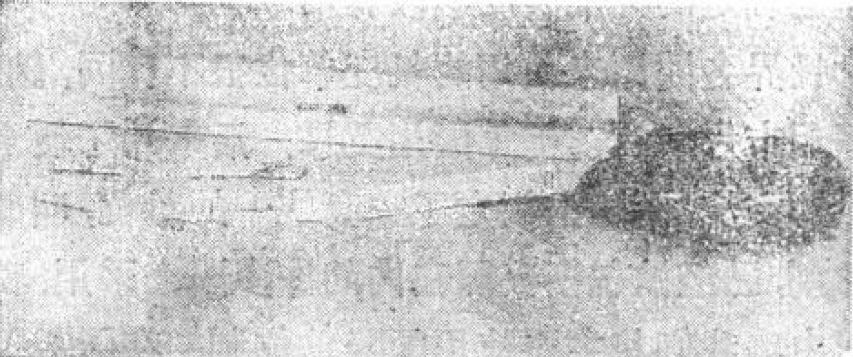
\includegraphics[width=0.5\textwidth]{../pic/czwl1-ch1-1}
    \caption{木尺,卷尺}\label{fig:1-1}
\end{figure}

测量长度的基本工具是刻度尺(图\ref{fig:1-1})。
用最小刻度是厘米的尺来测量,厘米下一位的毫米数要靠眼睛来估计,估计的数值就和真实的值有差异,所以测量只能准确到厘米。
用最小刻度是毫米的尺来测量,毫米下一位的数字要靠眼睛来估计,所以测量只能准确到毫米。
可见,\CJKunderwave{测量所能达到的准确程度是由刻度尺的最小刻度决定的}。

为了制作窗帘而测量窗户的长度,准确到厘米就足够了,为了安装玻璃而测量窗户的长度,就要准确到毫米,否则,
玻璃的大小跟窗框相差太多,就可能安装不上去。可见,\CJKunderwave{测量需要达到的准确程度跟测量的要求有关系}。

\begin{figure}[htbp]
    \centering
    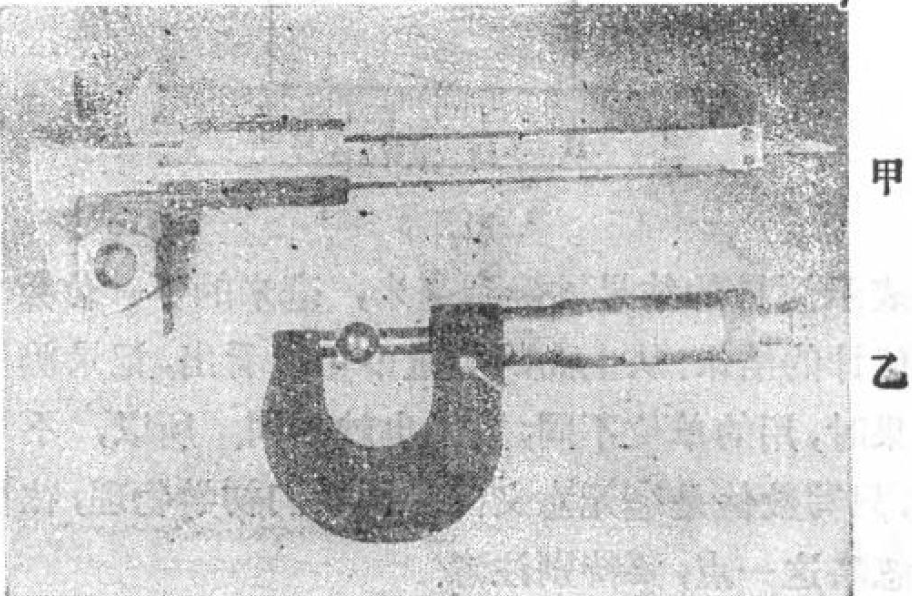
\includegraphics[width=0.5\textwidth]{../pic/czwl1-ch1-2}
    \caption{甲:游标卡尺 \hspace{1em} 乙:螺旋测微器}\label{fig:1-2}
\end{figure}

随着生产技术的发展,工业上对于某些产品或零件的测量,要求越来越严格,有时需要准确到 $0.01$ 毫米,
甚至需要准确到微米。一般最小刻度是厘米或毫米的尺就不能满足需要了,于是人们又研制出了一些精密的测量长度的工具,
游标卡尺( 图 \ref{fig:1-2} 甲) 测量的准确程度可以达到 $0.1$ 毫米、$0.05$ 毫米或 $0.02$ 毫米。
螺旋测微器,也叫千分尺( 图 \ref{fig:1-2} 乙),测量的准确程度可以达到 $0.01$ 毫米。
工厂里常常使用这两种测量工具。它们的原理和使用方法到高中将要学习。
除此以外,人们还制造出了各种光学测量仪器,用它们来测量长度,准确程度就更高了。
\CJKunderwave{在测量长度的时候,要先根据实际情况确定测量需要达到的准确程度,然后再根据要求选用适当的测量工具}。

\begin{figure}[htbp]
    \centering
    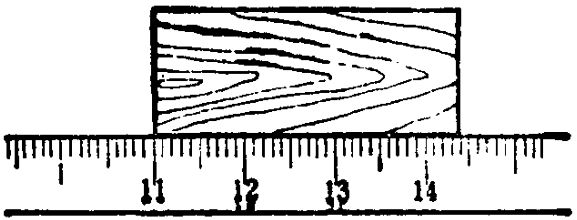
\includegraphics[width=0.5\textwidth]{../pic/czwl1-ch1-3}
    \caption{}\label{fig:1-3}
\end{figure}

\CJKunderwave{记录测量的结果,必须在数值后面写出所用的单位}。
例如,在图 \ref{fig:1-3} 所示的测量中,用的尺最小刻度是毫米,
如果用厘米作单位,木块的长度就是 $3.39$ 厘米,
如果用毫米作单位,木块的长度就是 $33.9$ 毫米。
这样写表示测量的结果准确到毫米,毫米的下一位数字 $9$ 是估计的结果。
从上面的测量中可以看出,记录测量的结果时,用的单位不同,数值也就不同。
所以,不写单位,只写数值是毫无意义的。
同学们初学物理,往往容易忽略这一点,要特别注意。

\begin{table}[H]
    \centering
    \caption*{一些距离和长度 (单位:米)}
    \begin{tabular}{w{l}{10em}w{r}{8em}}
        银河系的半径        & $6 \times 10^{19}$ \\
        太阳的半径          & $7 \times 10^8$ \\
        地球到月球的距离    & $3.8 \times 10^8$ \\
        地球的半径          & $6.4 \times 10^6$ \\
        月球的半径          & $1.7 \times 10^6$ \\
        一张纸的厚度        & $0.7 \text{~} 1 \times 10^{-4}$\footnotemark \\
        链球菌的半径        & $0.3 \text{~} 0.5 \times 10^{-6}$ \\
        原子的半径          & $0.5 \text{~} 3 \times 10^{-10}$ \\
    \end{tabular}
\end{table}
\footnotetext{$10^{-4}$ 是一种表示小数的科学记数法。这种记数法表示的意思是
$10^{-1} = 0.1$,
$10^{-2} = 0.01$,
$10^{-3} = 0.001$,…… ,
$0.7 \text{~} 1 \times 10^{-4}$ 就是 $0.00 \; 007$ ~ $0.0 \; 001$。
}


\nonumsection{阅读材料: 长度单位的发展过程}

长度的单位是可以任意规定的。从古到今,不同的国家,不同的时代,用过不同的长度单位。
古代,人们常常用身体的某些部分作为长度单位。
比如,我国古书《孔子家语》中有“布手知尺”的说法,意思是把张开的大拇指和中指两端间的距离作为 $1$ 尺。
埃及在建造金字塔的时候,曾经用肘到中指尖的距离作为长度单位。
英国曾经用从国王亨利第一的鼻尖到平伸手臂的手指尖的距离作为长度单位。
除此以外,古代还用某物品的长度作为长度单位,比如我国《汉书 \; 律历志》上记载着,以一粒黍的宽度作为 $1$ 分。
这类长度单位的缺点是长短不固定,造成测量上的混乱。

1791 年,法国决定把通过巴黎的子午线,从赤道到北极的长度的 $\dfrac{1}{10 \; 000 \; 000}$ (图 \ref{fig:1-4})作为长度单位,叫做米。
后来根据测量结果用纯铂制成了一个标准米原器,保存在法国档案局。


\begin{figure}[htbp]
    \centering
    \begin{minipage}{7cm}
    \centering
    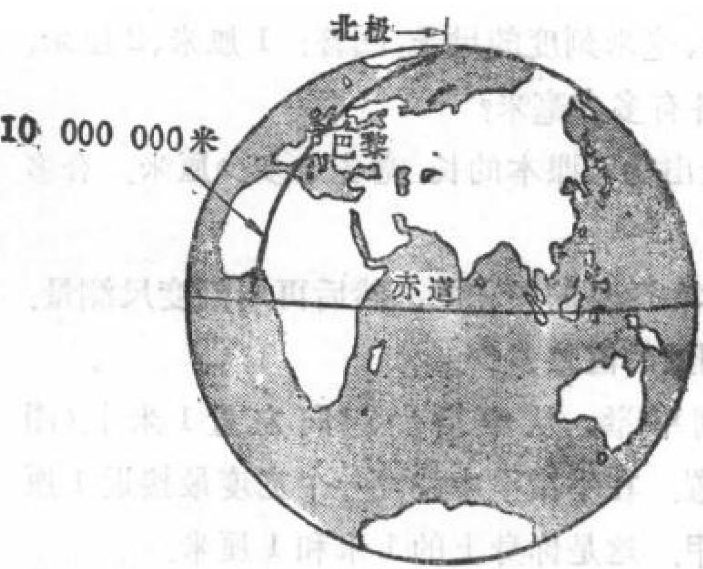
\includegraphics[width=4cm]{../pic/czwl1-ch1-4}
    \caption{}\label{fig:1-4}
    \end{minipage}
    \qquad
    \begin{minipage}{6cm}
    \centering
    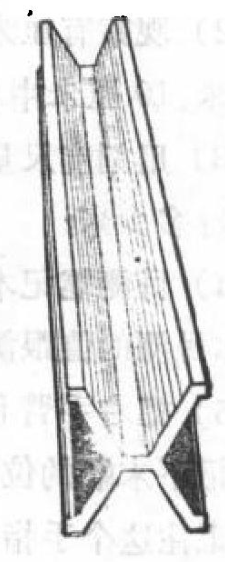
\includegraphics[width=1cm]{../pic/czwl1-ch1-5}
    \caption{国际米原器}\label{fig:1-5}
    \end{minipage}
\end{figure}


由于米的长度比较固定,优点比较多,陆续被许多国家采用。
1889 年用含 $90\%$ 的铂和 $10\%$ 的铱的合金制成了一个横截面是 X 形的国际米原器(图 \ref{fig:1-5}),
保存在法国巴黎的国际计量局里。在它的凹槽的两端分别刻着三条细线,温度是 0 ℃ 时,
两端的中间一条细线之间的距离是 $1$ 米。


用米作长度单位比用人体某些部分或某些物品作长度单位前进了一大步。但是,由于米原器天长日久会变形,
不能适应科学技术发展的更高耍求。 1960 年国际上决定用原子光谱来规定米的长度。

19 世纪 50 年代,在中法通商中米开始传入我国。现在我国已正式采用米作为长度单位。


\lianxi

(1) 在你的刻度尺上分别找出1 厘米、1 分来的长度, 并且画在作业本上。

(2) 观察有厘米、毫米刻度的尺子,回答: 1 厘米、2 厘米、$4.5$ 厘米、10 厘米中各有多少毫米?

(3) 用刻度尺量出物理课本的长、宽各是多少厘米。合多少分米? 多少米?

(4) 目测笔记本和课桌的长和宽,然后再用刻度尺测量。看看你目测的值跟测量的值差多少。

(5) 把右手臂侧平举,从中指尖起向左量 1 米长(图 \ref{fig:1-6}), 记下末端的位置。
在手指甲中找出一个宽度最接近 1 厘米的,记住这个手指甲。
这是你身上的 1 米和 1 厘米。

用你身上的 1 米测量教室的长和宽,并跟用卷尺测量的结果相比较。
用你身上的 1 厘米测量铅笔的长,并跟用刻度尺测量的结果相比较。

\begin{figure}[htbp]
    \centering
    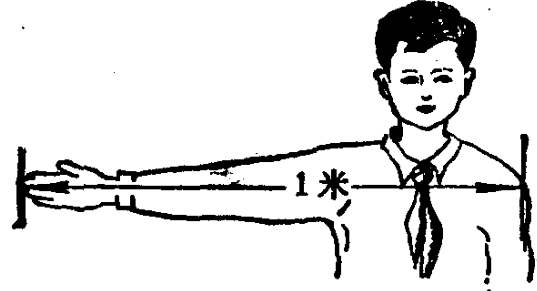
\includegraphics[width=0.3\textwidth]{../pic/czwl1-ch1-6}
    \caption{}\label{fig:1-6}
\end{figure}

(6) 人的身高早晨比晚上高。找一个人量一量,看看他早上比晚上高多少(用毫米作单位)。

(7) 地球的半径是 $6.4 \times 10^3$ 千米,合多少米?多少厘米?

(8) 地球到月球的距离是 $3.8 \times 10^8$ 米,合多少千米?


\section{长度测量的一些特殊方法}\label{sec:1-2}

长方形的长和宽、正方体的边长、圆柱体的高等直线长度,都可以用刻度尺直接测量。
铁路、公路、跑道等往往是弯曲的,曲线的长度怎么测量呢?
圆锥体的高虽然是直线,但是用刻度尺却很难测准。这又怎么办呢?
用有毫米刻度的尺无法直接测出一张纸的厚度,而我们要知道这个厚度,又没有更精密的尺,该怎么测量呢?

对于这些不能直接用刻度尺测出的长度,要根据具体情况想些特殊的方法。


\begin{figure}[htbp]
  \centering
  \begin{minipage}{9cm}
  \centering
  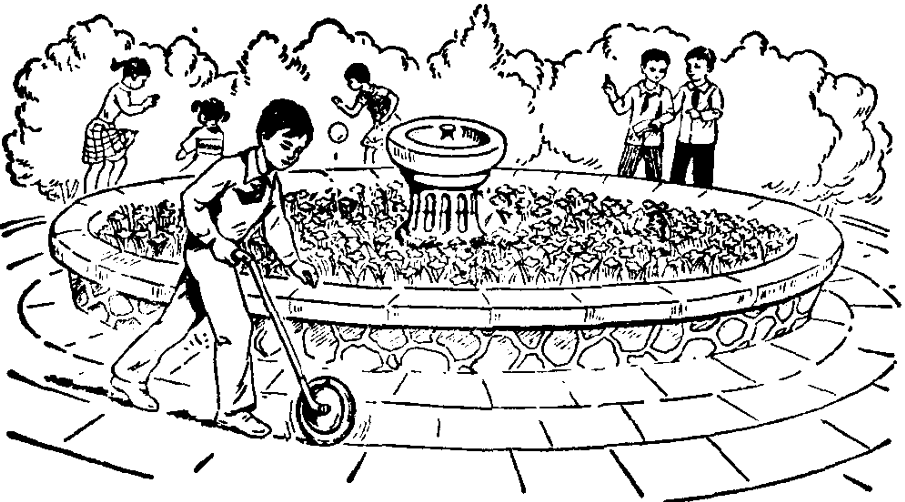
\includegraphics[width=9cm]{../pic/czwl1-ch1-7}
  \caption{}\label{fig:1-7}
  \end{minipage}
  \qquad
  \begin{minipage}{4cm}
  \centering
  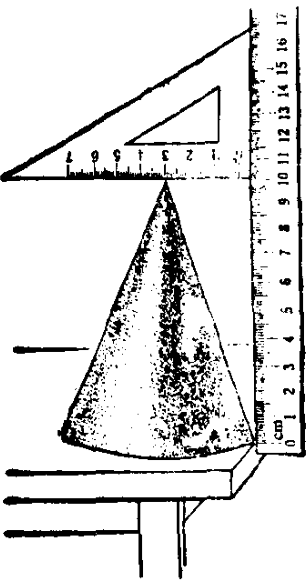
\includegraphics[width=3.5cm]{../pic/czwl1-ch1-8}
  \caption{}\label{fig:1-8}
  \end{minipage}
\end{figure}

曲线的长度可以用一个轮子沿着曲线滚动,测出轮子的周长,记下滚过的圈数,用轮子的周长乘以圈数,
就可以得到曲线的长度(图 \ref{fig:1-7})。火车、汽车上记录行驶路程的里程表,就是根据这个道理制做的。
比较短的曲线可以利用一条弹性不大的柔软棉线来测量。
先把棉线放在曲线上,让它跟曲线完全重合,在棉线上标出曲线的起点和终点,然后把棉线放直,
量出棉线上两点间的距离,就得到了曲线的长度。


圆锥体的高可以照图 \ref{fig:1-8} 那样,用直角三角板和刻度尺配合进行测量。

用有毫米刻度的尺测不出一张纸的厚度,也测不出两张纸的厚度,但是能测出 100 张纸的厚度。
把测出的厚度除以总张数,就得到一张纸的厚度。

\lianxi

(1) 用有毫米刻度的尺,近似地量出练习本里一张纸的厚度。

(2) 用刻度尺和三角板测量乒乓球的直径(图 \ref{fig:1-9})。


\begin{figure}[htbp]
  \centering
  \begin{minipage}{6cm}
  \centering
  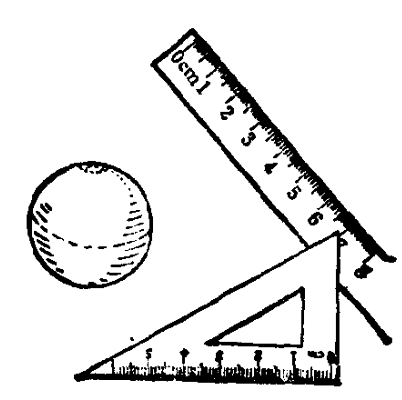
\includegraphics[width=6cm]{../pic/czwl1-ch1-9}
  \caption{}\label{fig:1-9}
  \end{minipage}
  \qquad
  \begin{minipage}{4cm}
  \centering
  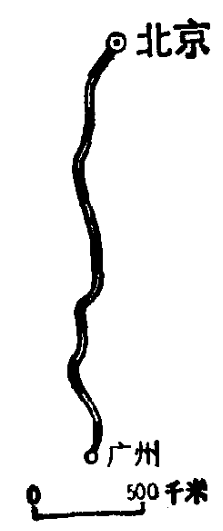
\includegraphics[width=2.5cm]{../pic/czwl1-ch1-10}
  \caption{}\label{fig:1-10}
  \end{minipage}
\end{figure}

(3) 测量图 \ref{fig:1-10} 中京广铁路线的近似长度(用千米作单位)。

(4) 先用刻度尺量出你步行时两脚间的距离,即一步的长度,然后测出篮球场的长和宽各是多少步,
再算出篮球场的长度和宽度。


\nonumsection{小实验: 测量细金属丝的直径}

找一支圆铅笔,一把有毫米刻度的尺,一段长 50 厘米左右的细金属丝。
想办法用刻度尺量出细金属丝的直径。



\section{误差}\label{sec:1-3}

\begin{figure}[htbp]
  \centering
  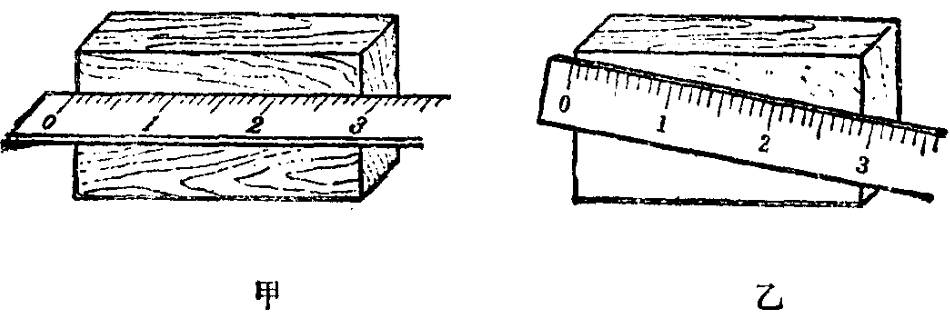
\includegraphics[width=0.6\textwidth]{../pic/czwl1-ch1-11}
  \caption{}\label{fig:1-11}
\end{figure}

测量的时候,如果测量方法不正确,就会产生错误。
使用刻度尺量长度时,必须注意:在用厚刻度尺的时候,尺要照图 \ref{fig:1-11} 甲那样放置,
使刻度贴近被测物体,这样容易看准物体的边线所对的刻度值。
刻度尺在被量物体上的位置不要象图 \ref{fig:1-11} 乙那样歪斜。
观察刻度线的时候,视线要跟尺垂直(图 \ref{fig:1-12})。

\begin{figure}[htbp]
  \centering
  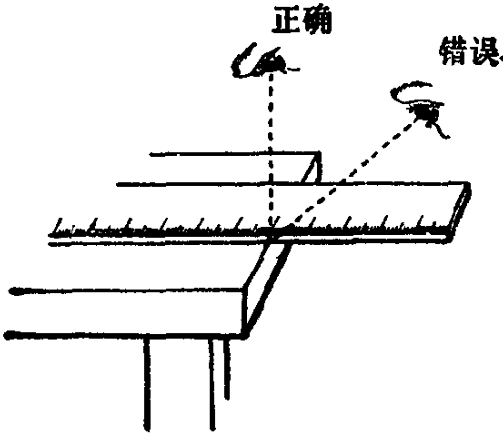
\includegraphics[width=0.4\textwidth]{../pic/czwl1-ch1-12}
  \caption{}\label{fig:1-12}
\end{figure}

两个同学都用正确的测量方法,认真、仔细地测量同一枝铅笔的长度,而测出的结果可能并不完全相同。
但是,一个物体的真实长度总是一定的,我们把物体的真实长度叫做它的真实值。
一般说来,测量值和真实值之间总会有些差异,这个差异叫做\textbf{误差}。
误差和错误不同,错误是应该而且可以避免的,而误差是不能绝对避免的。
误差是怎么产生的呢?

误差的产生跟测量工具有关系。例如刻度尺的刻度不够准确,钢尺的热胀冷缩,还可能有些弯曲,
用它们测长度就会产生误差。测量工具越精密,误差就越小。

误差的产生还跟测量的人有关系。我们知道,用最小刻度是毫米的尺量长度,毫米的下一位数字是估计出来的。
不同的人在估计的时候,有的人估计得偏大些,有的人估计得偏小些。
用秒表测时间的时候,有的人按得早些,有的人按得晚些。
这就产生了跟测量的人有关系的误差。

由于测量时要有估计,所以一个人用同一个测量工具对一个物体测量几次,所得的结果也会不同。
比如一位同学用有毫米刻度的尺先后五次测量一个物体的长度,各次测得的数值分别为

$l_1 = 1.41$ 厘米,$l_2 = 1.42$ 厘米,$l_3 = 1.42$ 厘米,$l_4 = 1.41$ 厘米,$l_5 = 1.43$ 厘米。

各次测得的数值相近,不能说哪一次测量更准确。但是可以想到,有时测量值大于真实值,有时测量值小于真实值,
而多次测量的平均值会更接近真实值,误差较小。因此,我们取五次测量的平均值 $\bar{l}$ 作为测量结果。

$\begin{aligned}[t]
    l &= \dfrac{l_1 + l_2 + l_3 + l_4 + l_5}{5} \\
      &= \dfrac{1.41 \,\text{厘米} + 1.42 \,\text{厘米} + 1.42 \,\text{厘米} + 1.41 \,\text{厘米} + 1.43 \,\text{厘米}}{5} \\
      &= \dfrac{7.09 \,\text{厘米}}{5} = 1.42 \,\text{厘米 。}
\end{aligned}$

误差是不能绝对避免的,但是随着科学技术的发展,精密测量仪器不断出现,
实验方法不断改进,人们减小误差的本领越来越大。
例如,过去用几何方法测量地球到月球的距离,误差有几千米,现在用激光来测,误差就只有几厘米了。

在学习物理的过程中,要做许多实验。做实验的时候,一定要认真、细致,不要出错误。
同时还应该注意分析误差产生的原因,想办法来减小它,提高自己的实验技能。



\section{实验:测量圆的周长和直径}\label{sec:1-4}

\shiyan{目的} 测量圆的周长和直径, 练习使用刻度尺。

\shiyan{器材} 刻度尺,三角板,纸条,圆柱体,针。

\shiyan{步骤}

(1) 把纸条紧包在圆柱体的侧面上,在纸条重叠处用针扎个孔。
然后把纸条展开,用刻度尺测量两孔之间的距离(圆的周长)。
这样做三次,把数值填入表内,算出平均值。

(2) 想办法用刻度尺、三角板量出圆柱体的直径(圆的直径)。
在圆周的不同位置处测量三次,填入表内,算出平均值。

\begin{table}[H]
    \centering
    \renewcommand\arraystretch{1.5}
    \begin{tabular}{|w{c}{8em}|*{3}{w{c}{4em}|}w{c}{5em}|}
        \hline
        实验次数        & 1 & 2 & 3 & 平均值  \\ \hline
        圆的周长(厘米) &   &   &   &  \\ \hline
        圆的直径(厘米) &   &   &   &  \\ \hline
    \end{tabular}
\end{table}

\shiyan{作业} 用测得的圆的周长和直径的平均值计算 $\pi$ 值。


\section{质量}\label{sec:1-5}

空气、水、铜、铁、木材、胶等都是物质,所有的物体,比如桌子、椅子、飞机、轮船都是由物质组成的。
物体里所含的物质有多有少,一桶水比一杯水所含的水多,大铁块比小铁棒所含的铁多。
为了说明物质的多少,物理学里引入了\textbf{质量}这个物理量。

\textbf{物体所含物质的多少叫做质量}。

把一块铁轧成铁片,形状变了,但所含铁的多少没有变。也就是质量没有变。
一块冰融化成水,由固体变成了液体,物质的状态变了,但所含水的多少没有变,质量也就没有变。
可见,\CJKunderwave{质量是物体本身的一种属性},它不随物体的形状、温度、状态而改变。
质量也不随物体的位置而改变。
一罐头水果,不论把它放在赤道还是北极,罐头里水果的多少都不会改变,所以质量也不会改变;
就是被宇航员带到月球上,质量也不会改变。


\begin{wrapfigure}[13]{r}{7cm}
    \centering
    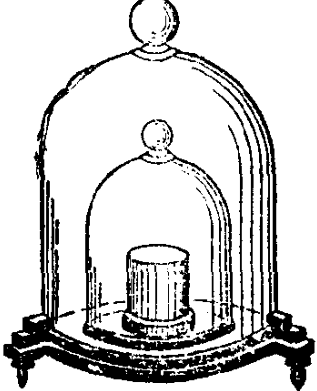
\includegraphics[width=0.2\textwidth]{../pic/czwl1-ch1-13}
    \caption{国际千克原器}\label{fig:1-13}
\end{wrapfigure}


在日常生活中,人们经常要测量物质的质量。
比如我们买柴、买米,总要用秤称一称,称的就是柴和米的质量。
在科学技术中也要经常测量质量。

为了测量物体的质量,需要定出质量的单位。在国际单位制里,质量的主单位是\textbf{千克}(也叫公斤)。
原来人们规定在 $4\celsius$ 时 1 升纯水的质量为 1 千克。
后来根据这个规定,用铂铱合金制成一个质量是 1 千克的圆柱体,作为 1 千克的标准,叫做国际千克原器(图 \ref{fig:1-13}),保存在法国巴黎的国际计量局里。
为了测量质量很小的物体,还规定了比千克小的单位——克和毫克,
\vspace{-1em}\begin{center}
    \begin{tabular}{l}
        1 千克 = 1000 克, \\
        1  克 = 1000 毫克。 \\
    \end{tabular}
\end{center}\vspace{-1em}
测量质量较大的物体时,通用用吨作为单位,

\centerline{1  吨 = 1000 千克。}

\begin{table}[H]
    \centering
    \caption*{\textbf{一些物体的质量} (单位:千克)}
    \begin{tabular}{w{l}{10em}w{r}{8em}}
        银河系      & $2.8 \times 10^{41}$ \\
        太阳        & $2.0 \times 10^{30}$ \\
        地球        & $6.0 \times 10^{24}$ \\
        月球        & $7.4 \times 10^{22}$ \\
        尘埃微粒    & $6.7 \times 10^{-10}$ \\
        青霉素分子  & $5.0 \times 10^{-17}$ \\
        氢原子      & $1.7 \times 10^{-27}$ \\
        电子        & $9.1 \times 10^{-31}$ \\
    \end{tabular}
\end{table}

\,

\section{质量的测量 \quad 天平}\label{sec:1-6}

在日常生活中我们可以看到许多称物体质量的工具。
比如在仓库和火车站可以看到能称很大质量的磅秤,
在商店可以看到使用方便的托盘秤和杆秤,
在药房和实验室可以看到能够精确地称质量的天平。
测量质量的工具很多,使用的时候,要根据需要适当地选用。

\begin{figure}[htbp]
    \centering
    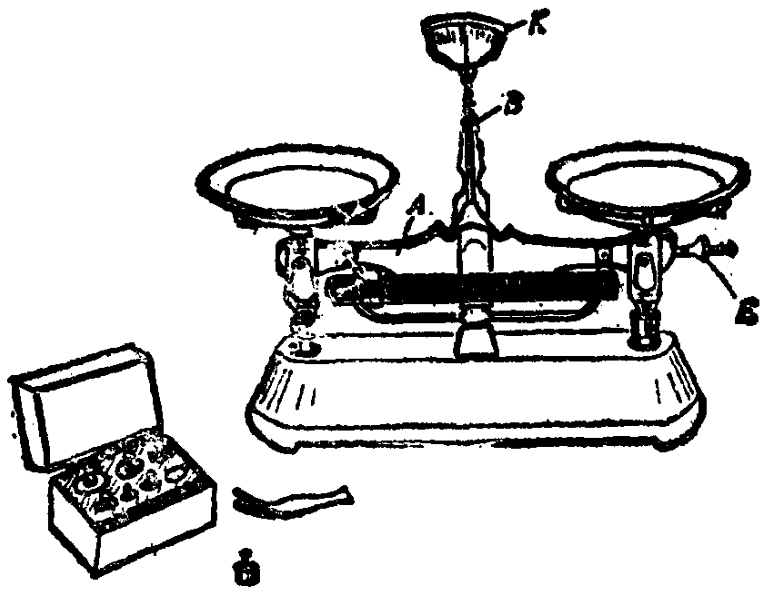
\includegraphics[width=0.6\textwidth]{../pic/czwl1-ch1-14}
    \caption{托盘天平和砝码}\label{fig:1-14}
\end{figure}

图 \ref{fig:1-14} 是实验室里常用的托盘天平。横梁 $A$ 可以自由摆动。
如果放在两个天平盘里的物体的质量不相等,质量较大的那端横梁就下沉。
\CJKunderwave{只有两个盘里的质量相等,横梁才停在水平位置,或者说横梁平衡了}。
天平就是根据这个道理来称物体质量的。

每架天平都配有一套砝码作为标准质量,装在砝码盒里,天平横梁上还附有标尺。
移动标尺上的游码相当于向天平盘里加小砝码。

使用托盘天平时,\CJKunderwave{应把天平放在水平桌面上}。
先把游码放在标尺左端的 “0” 点上,然后旋动横梁右端的调节螺母 $E$,
使指针 $B$ 对准刻度盘 $K$ 的中央,这就表示横梁平衡了。

测量的时候,把被测物体放在左盘里。估计被测物体的质量,选择适当的砝码放在右盘里。
如果右盘下沉,指针偏向刻度盘的右侧,这表示砝码的质量大了,可换用较小的砝码。
如果右盘上翘,指针偏向刻度盘左侧,就表示砝码的质量小了,可增加砝码,
并调节游码的位置,直到指针指在刻度盘的中央,横梁平衡为止。
这时盘里砝码的总质量加上游码所对的刻度值,就等于被测物体的质量。

天平是比较精密的仪器,使用要十分精心。
不要用手摸天平盘,更不准把潮湿的东西或化学药品直接放在天平盘里。
砝码要用镊子夹取,不准用手拿。
往盘里加减砝码要轻拿轻放,用后要及时放回砝码盒里,不要随意放置。
要注意保持天平和砝码干燥、清洁,防止锈蚀。
每架天平都有一定的称量范围,加在天平上的质量不能超过它的称量范围,否则会损伤天平。


\section{实验:用天平称物体的质量}\label{sec:1-7}

\shiyan{目的} 学习用托盘天平称物体的质量。

\shiyan{器材} 托盘天平,砝码,几个相同的硬币(或者几个相伺的钮扣),铁块, 1 厘米长的一段棉线。

\shiyan{步骤}

(1) 调节天平横梁右端的螺母,使横梁平衡。

(2) 把铁块放在左盘里,先根据估计,用镊子往右盘里试加砝码,然后移动游码,直到横梁平衡。

(3) 横梁平衡后,计算砝码的总质量并观察游码所对的刻度值,得出所称的铁块的质量。

(4) 称量完毕,把砝码全部放回盒内,不要遗漏。

(5) 把几个相同的硬币放在左盘里,称出它们的总质量。

(6) 求出一个硬币的质量的平均值。

(7) \mylabel{celiang-keben-zhiliang}称出物理课本的质量,并把它记在\pageref{shiyong-keben-zhiliang} 页 \hyperref[shiyong-keben-zhiliang]{第 (4) 题} 的后边。

\shiyan{观察与思考}

(1) 将 1 厘米长的棉线放在天平左盘里,称称看,能称出它的质量来吗?想一想,用什么办法能够测出 1 厘米长的棉线的质量?

(2) 想想看,怎样用天平称液体的质量。

\lianxi

(1) 一个同学为了验证冰融化成水后质量不变,他先测出了冰的质量,然后把冰放入一个开口的烧瓶里加热,直到水沸腾了,他才去测量水的质量。
可是测量的结果表明水的质量减小了,你能找出质量减小的原因吗?

(2) 考古学家研究了一种恐龙化石后,认为这种恐龙活着时质量大约有 50 吨。一只恐龙的质量相当于多少个 50 千克的人的质量?

(3) 有一堆同一规格的小零件,每个只有几十毫克,估计有几千个。
手边有一架天平,你能利用它很快知道这堆零件的确切数目吗?用具体的数字例子来说明你的办法。


\nonumsection{复习题}\label{sec:1-fuxi}

(1) 常用的测量长度的工具是什么?在长度测量中,测量的准确程度由什么决定?
如果刻度尺上的最小刻度是厘米,用这把刻度尺测量,能准确到什么程度?
如果用米作单位来记录测量结果,测量值的小数点后面应该有几位数字?哪一位数字是估计的?

(2) 什么叫做物体的质量?为什么说质量是物体本身固有的一种属性?

(3) 在国际单位制中,长度、质量的主单位是什么?它们的常用单位还有哪一些?

(4) 怎样调节托盘天平?使用时要注意些什么?

(5) 在测量的时候,应该怎样选择适当的测量工具?

(6) 什么叫误差?误差是怎样产生的?


